\documentclass{beamer}

\mode<presentation>
{
  \usetheme{Madrid}      % or try Darmstadt, Madrid, Warsaw, ...
  \setbeamertemplate{navigation symbols}{}
  \setbeamertemplate{caption}[numbered]
} 

\colorlet{beamer@blendedblue}{black}

\usepackage[french]{babel}
\usepackage[utf8x]{inputenc}
\usepackage[T1]{fontenc}
%\usepackage[squaren,cdot]{SIunits}
\usepackage{graphicx}
\usepackage{listings}
\usepackage{wrapfig}

\graphicspath{}

\logo{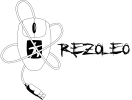
\includegraphics[height=0.8cm]{rezoleo.png}\vspace{10pt}\hspace{20pt}}
\title{Couche réseau - Adressage}
\author{LEDER "Ziman" Simon}
\institute{Rezoleo\\}
\date{\today}

\begin{document}
	
	\maketitle

	\begin{frame}
		\frametitle{Sommaire}
		\tableofcontents
	\end{frame}

\section{Introduction}
	\begin{frame}{Introduction}{Définition}
		La couche réseau a pour rôle général de faire transiter des données entre deux points d'un réseau (émetteur et récepteur). Ses fonctions principales concernent l'adressage, la constitution des trames de niveau 4 et les techniques de routage.
		\begin{figure}
			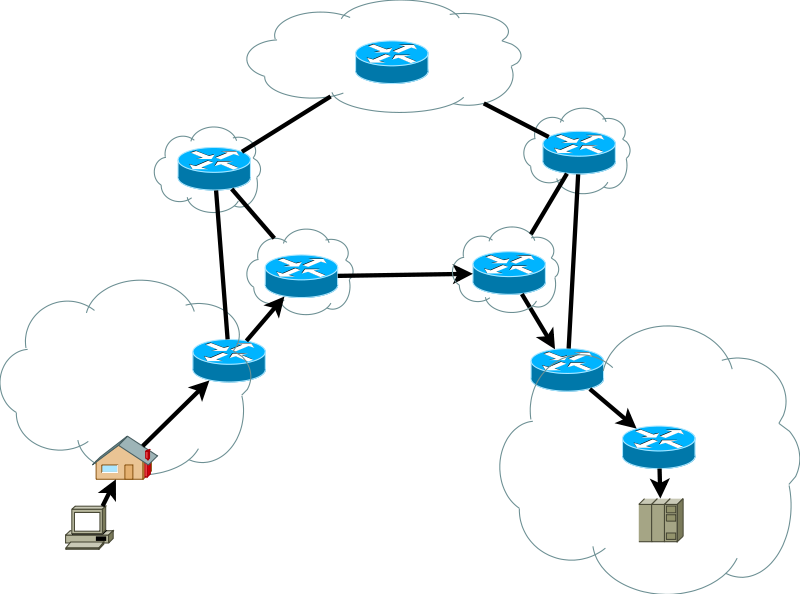
\includegraphics[scale = 0.2]{router.png}
		\end{figure}
	\end{frame}

	\begin{frame}{Introduction}{Définition}
		\begin{itemize}
			\item[\textbullet] Un adressage doit être mise en place de façon à identifier de manière unique tous les éléments actifs (ordinateurs, périphériques, éléments de routage...). 
			\item[\textbullet] Le transport de la trame de l'émetteur au récepteur nécessite une détermination du chemin à emprunter: c’est le routage. Si un émetteur envoie plusieurs trames à un même destinataire toutes n'emprunteront pas forcément le même chemin.
		\end{itemize}
	\end{frame}

	\begin{frame}{Introduction}{Routage}
		Le routage est le mécanisme par lequel des chemins sont sélectionnés dans un réseau pour acheminer les données d'un expéditeur jusqu'à un ou plusieurs destinataires.\\
		\begin{figure}
			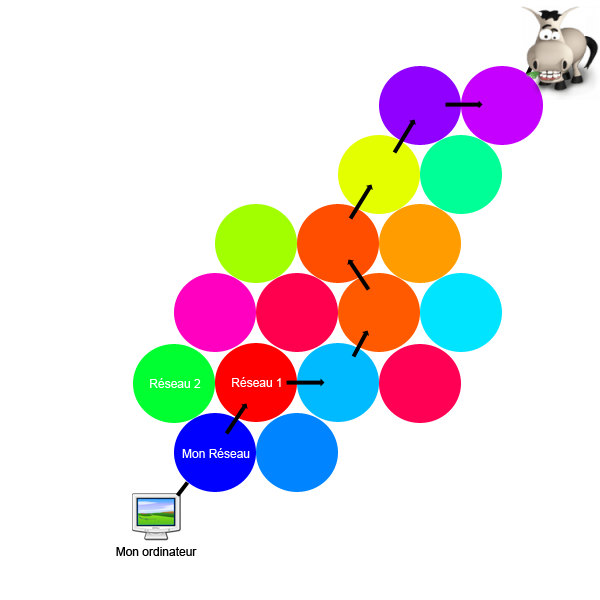
\includegraphics[scale = 0.3]{routage.png}
		\end{figure}
	\end{frame}

	\begin{frame}{Introduction}{Sigles}
		\begin{itemize}
			\item[\textbullet] IP signifie Internet Protocol : littéralement "le protocole d'Internet". C'est le principal protocole utilisé sur Internet.
			\item[\textbullet] Internet signifie Inter-networks, c'est à dire "entre réseaux". Internet est l'interconnexion des réseaux de la planète.
		\end{itemize}
			Le protocole IP permet aux ordinateurs reliés à ces réseaux de dialoguer entre eux.
	\end{frame}

\section{Adressage}

	\begin{frame}{Adressage}{késséssé}
		Une adresse IP est un numéro d'identification qui est attribué à chaque branchement d'appareil à un réseau informatique utilisant l'Internet Protocol.\\
		Il existe des adresses IP de version 4  IPv4 et de version 6 IPv6.\\
		Exemple : 212.85.150.134 
	\end{frame}

	\begin{frame}{Adressage}
		Le protocole IP détermine le destinataire du message grâce à 3 champs :
		\begin{itemize}
		\item[\textbullet] Le champ adresse IP : adresse de la machine
		\item[\textbullet] Le champ masque de sous-réseau : un masque de sous-réseau permet au protocole IP de déterminer la partie de l'adresse IP qui concerne le réseau
		\item[\textbullet] Le champ passerelle par défaut : Permet au protocole Internet de savoir à quelle machine remettre le datagramme si jamais la machine de destination n'est pas sur le réseau local. 
		\end{itemize}
	\end{frame}

	\begin{frame}{Adresse}{Masque}
		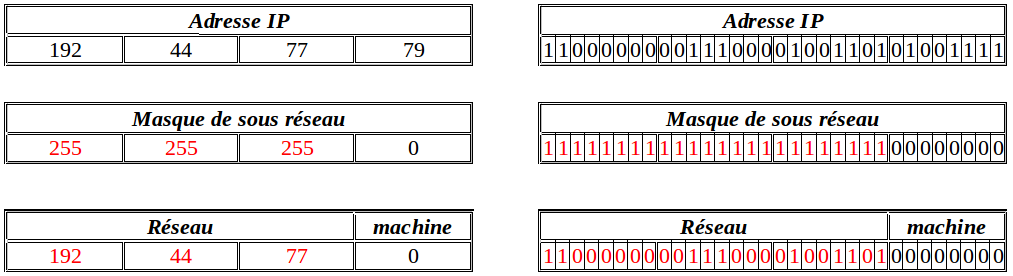
\includegraphics[scale=0.33]{masque.png}
	\end{frame}

	\begin{frame}{Adresse}{Adressage CIDR}
	\begin{center}
		192.44.77.79/24
	\end{center}
	\end{frame}

\section{routage}

	\begin{frame}{Routage}{}
		\begin{figure}
			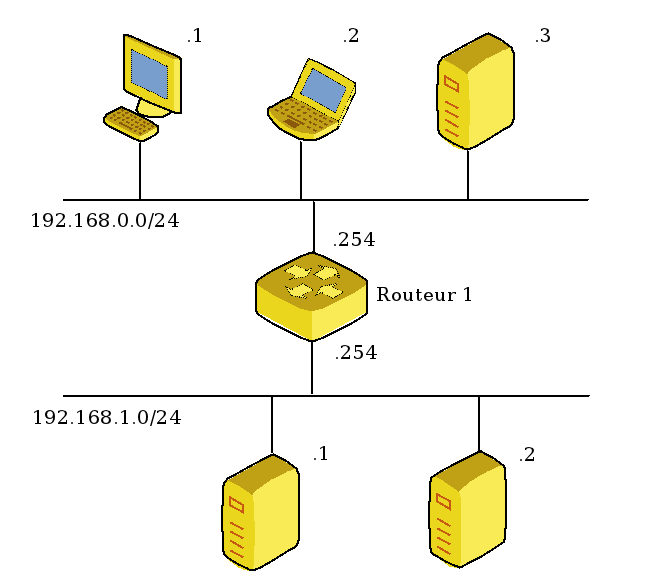
\includegraphics[scale=0.4]{Network.png}
		\end{figure}
	\end{frame}
	

	\begin{frame}{DHCP}{}
		\begin{figure}
			Dynamic Host Configuration Protocol (DHCP) est un terme anglais désignant un protocole réseau dont le rôle est d’assurer la configuration automatique des paramètres IP d’une station, notamment en lui affectant automatiquement une adresse IP et un masque de sous-réseau.\\
			DHCP de la rez : 172.30.128.40
		\end{figure}
	\end{frame}

	\begin{frame}{ARP}{}
		\begin{figure}
			L’Address Resolution Protocol (ARP, protocole de résolution d’adresse) est un protocole utilisé pour traduire une adresse de protocole de couche réseau (typiquement une adresse IPv4) en une adresse MAC (typiquement une adresse Ethernet), ou même de tout matériel de couche de liaison.
		\end{figure}
	\end{frame}

	\begin{frame}{DNS}{}
		\begin{figure}
			Le DNS transforme l’adresse IP en un nom en utilisant un serveur de nom de domaine situé dans le réseau Internet). L’attribution du nom de domaine est payant. La plupart des adresses IP peuvent être converties en un nom de domaine et inversement. Le nom de domaine est plus facilement lisible : fr.wikipedia.org est le nom de domaine correspondant à 91.198.174.2
		\end{figure}
	\end{frame}
	
	\begin{frame}{Table de routage}{}
		\begin{figure}
			Exemple de table
		\end{figure}
	\end{frame}


\end{document}